\section{Technical Description of the application}

This section will explore the technical aspects of the application. This is done via a data flow, and separating the system into an MVC-architecture. 

\subsection{Application Structure}
\begin{itemize}
\setlength{\itemsep}{0.1em}
    \item \textbf{Parser}: The parser has the job of parsing and structuring the .OSM data, into individual classes. This component goal is to pass the parsed and structured .OSM data onto the next component. 
    \item \textbf{Data processing}: After the data has been parsed, the data needs to be processed. This component's goal is to further structure the data to be able to handle the data in an efficient way, so the newly structured .OSM data efficiently can be drawn to the user.
    \item \textbf{Visuals}:  The visual component controls all the components that are displayed to the user and drawn from the different parsed objects. The goal of the view component is to display the right data to the user and manage the logical states of the JavaFX elements.
\end{itemize}

\subsection{Data Flow}
\begin{figure}[ht]%
  \centering
  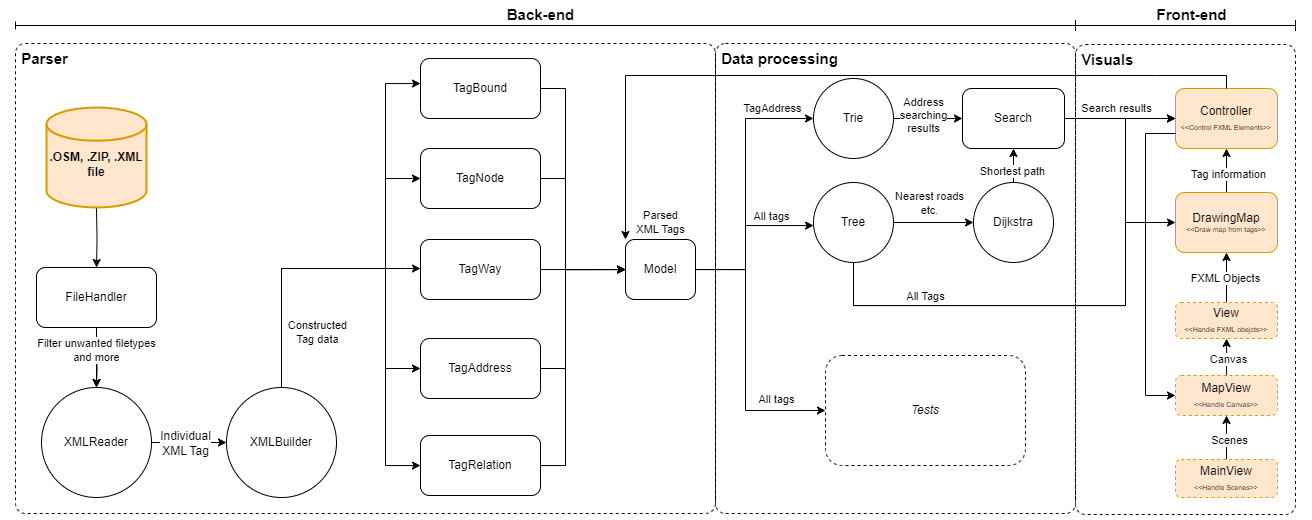
\includegraphics[width=14.5cm]{docs/material/dataflow.png}%
  \caption{\centering Flowchart of the flow of data in the application}\label{dataflow}%
\end{figure}\\
\subsubsection{Parser}\label{section/parser}
The parser is the first of the three smaller structural components to handle the inputted .OSM data. Firstly the data passes through the FileHandler to check inputted files for unsupported file types, unzips inputted .ZIP files and more. When accepted, the .OSM data is passed onto the \textit{XMLReader} file. The XMLReader extracts individual XML elements to be read by the \textit{XMLBuilder}, which reads the element and parses the data into objects. When the XML elements attributes and subtags have been read and parsed, all the data go into their respective Tag classes [see \ref{DataSet}]. 
It would also be in this step where the constructed Tag class would be appended to the binary pool, to be written into chunks. See \ref{DiscussionChunks} for the implementation.
\begin{itemize}
    \item Model class: intentional design to be a main exit point for all the parsed data, and an entry point to write the parsed data to binary. 
 
\end{itemize}

\textbf{Tags}\\
Every .OSM XML element has specific characteristics that can be split into five \textit{Tag’}s. All of the tag classes inherit from the abstract superclass \textit{Tag}, which handles common attributes and methods for all tags.
Each of the tags was implemented with the intention of being used in chunks. This has some major drawbacks when it comes to Minion Maps current implementation, without the functionality of chunks (see \ref{DiscussionChunks}).

\textbf{TagBound}\\
The \textit{TagBound }class represents the \textit{bounds }element in the .OSM file. The bounds element is the first .OSM element in the file. The bounds define a rectangular area of \textit{maximum, minimum }latitude and longitude. All of the XML elements that have their latitude and longitude are within the area that is within the .OSM file. There are only a few exceptions where there are references to XML elements that are without the bound area, this mostly occurs in the way and relation elements.

Minion map uses this class in both for the functionality to pan and zoom on the map, but was also supposed to be used as a header for chunk files to define the bound area.

\begin{figure}[ht]%
  \centering
  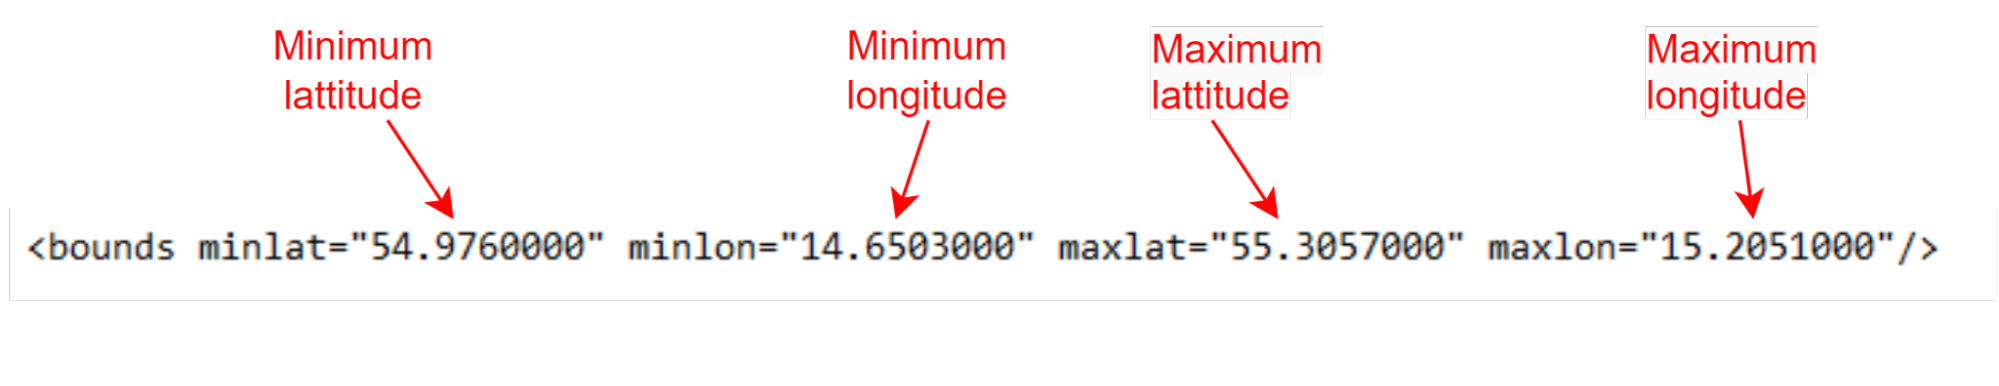
\includegraphics[width=15.5cm]{docs/material/TagBoundParse.png}%
  \caption{\centering Illustration of TagBounds when parsing}\label{tagNode}%
\end{figure}\\
\newpage
\textbf{TagNode}\\
\begin{figure}[ht]%
  \centering
  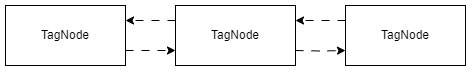
\includegraphics[width=12.5cm]{docs/material/TagNode.png}%
  \caption{\centering Illustration of TagNodes representation}\label{tagNode}%
\end{figure}\\
\textit{TagNode }is a class that represents a \textit{node }element in the .OSM file and is a sign point on the map. The node has a unique id and a latitude and longitude as attributes. 

In Minion Map we have made the TagNode compatible to be used as a double linked list, for the benefit of linking all of the nodes together if they are a part of a \textit{TagWay}.  

\textbf{TagWay}\\
\begin{figure}[ht]%
  \centering
  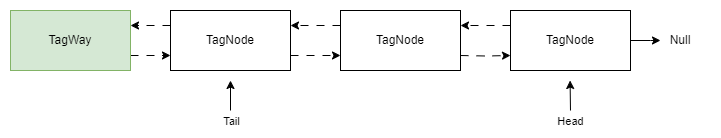
\includegraphics[width=14.5cm]{docs/material/TagWay.png}%
  \caption{\centering Illustration of TagWays representation}\label{TagWay}%
\end{figure}\\
\textit{TagWay }represents the \textit{way }tag in the .OSM file and is used to display lines or polygons. A TagWay is constructed via a sequence of TagNodes. The TagWay itself does not contain latitude or longitude, however, its referred TagNodes, implicitly defines where the TagWay is drawn. The TagWay is stored in memory as a linked element for the tail TagNode that the way represents.

A TagWay also contains a \textit{Type}, which defines whether the way should be a line or polygon, which layer and hierarchy it should be drawn on, and what color it should be drawn with.
\newpage
\textbf{TagAddress}\\
\textit{TagAddress }is similar to the native nodes, but the node has a series of subtags that contain the information of an address. 

In Minion Map, each node with the right subtags is parsed as an address to be later used in Trie and the KDTree. The reason to parse this kind of node into its own class is to ensure easy use throughout the application and fast instance checking of the class. \\

\textbf{TagRelation}\\
\begin{figure}[ht]%
  \centering
  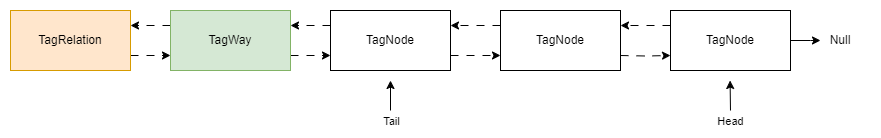
\includegraphics[width=14.5cm]{docs/material/TagRelation.png}%
  \caption{\centering Illustration of TagRelations representation}\label{TagRelation}%
\end{figure}\\
TagRelations are similar to TagWays, however instead of containing a list of \textit{TagNodes,}TagRelations contain a list of \textit{TagWays}. TagRelations can be a set of larger polygons ”multipolygons”, or it can be a network in for example public transport.

The TagRelation is stored as a link to a TagWay, just as the TagWay is linked to the tail TagNode in the list of referenced nodes. 

In Minion Map, TagRelations are only parsed if they are polygons. The list of TagWays are typically set up as either inner or outer ways. The entire collection of outer ways represents the larger polygon(s). The inner ways are polygons which are within the outer polygons. These inner ways are typically a completely normal TagWay as represented above. The outer TagWays however do not contain a type themselves. Instead, these should inherit the type of the relation.

\textbf{MecatorProjection}\\
One of our design choices was to project everything using Mercator projection. Due to some of the data being delivered in OSM as degrees which would mean that if anything distance related was required it would have to be converted by calculation in runtime. That led us to implementing this. With Mercator projections we already translate the necessary data in the loading phase. By calling the projection function in the parsing process and then storing the processed data inside of the heap instead.

\subsection{Data Processing}

\subsubsection{All Tags}
In order for the program to run smoothly. It is necessary that all of the tags can be obtained quickly, since we may end up working with millions of tags at once. Thankfully, since a computer screen only can be up to a certain size, only a selected number of tags need to be handled at once, the tags that appear on the screen. Since all tags implicitly or explicitly contain coordinates. The tags can be set up in a \textit{Tree} (see \ref{KDTree}), which sorts the objects based on their latitude and longitude.

This \textit{Tree} can also be used by the pathfinding algorithm \textit{Dijkstra}, to determine which roads or addresses are close to each other.

\subsubsection{Tag Addresses}
Defines the addresses for all the buildings on the map. This data needs to be processed, so that the user can search on these addresses. Additionally the program needs to be capable of auto completing the user’s input into a valid address. That’s why the Trie algorithm is implemented, which consists of “TrieNodes”, constructed by all the TagAddresses individual characters (see \ref{Trie}). 


\subsection{Visuals / Frontend}

Visuals is the part of the program that is responsible for everything that the user experiences while traversing the map. Here, both \textbf{view }and \textbf{controller }in our Model-View-Controller-architecture reside (MVC-architecture). The model is solely responsible for the entirety of backend processes. 
When working with the frontend, it is important for the view and controller to give and receive information to each other. Whenever the user \textit{controls }by panning over the map, information will be sent to MapView about whether a button should be marked blue, or a new tab should be opened. Whenever the view gets changed, the controller will have to behave differently to the modified interface. The controller also sends information back to the model, where data once again can be processed through the different algorithms.
For example, whenever the user \textit{controls }by panning over the map, the model needs to know how much the screen has changed in its position. Then the model will use that information to obtain which new polygons and lines should be drawn and which should not. This information will inevitably have an impact on what the user \textit{views }on the screen. 

\subsubsection{View}

The View class is a super class with two child-classes Lobby- and Mapview bound up to it. Each holds crucial information for the two screens that reside inside of the program: the start screen and map screen. Each view-class has its own controller, lobbyview: Start Screen Controller and MapView:Controller. 

The lobby view stores information such as what map the user wants to load, when pressing the button “Launch Map”, it sets the model object to a new instance of it from the file chosen by the user which is then created in the superclass View. 

The superclass View is also responsible for changing Views, loading their controller, fxml sheets and then storing protected data from the child classes in itself. Ensuring the data is only retrievable from the View-class itself which is the active data.

 \subsubsection{DrawingMap}
 The DrawingMap class is mainly responsible for the cartography itself. This means that it obtains all relevant polygons or lines (TagWays) and displays them appropriately by getting their individual types and their points (TagNodes).
The TagNode’s points are handled with the help of JavaFX’s transform. This ensures that the coordinates are handled differently with each frame, as the viewport gets panned and zoomed by the user.